
\begin{figure}[H]
	\centering
	\captionsetup{font=footnotesize}
	\begin{subfigure}{00.32\textwidth}
		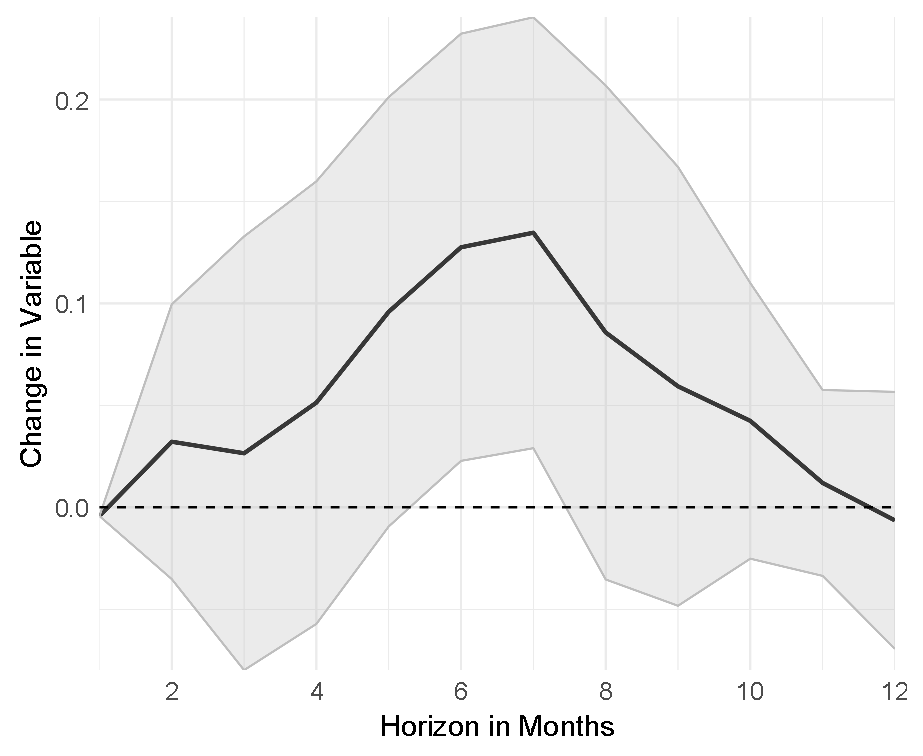
\includegraphics[width=1\textwidth]{output/lp/baseline/bHP/government_spending/government_spendingonexpectations1y_djn.eps}
		\caption{Government spending on 1-year}
	\end{subfigure}
	\begin{subfigure}{00.32\textwidth}
		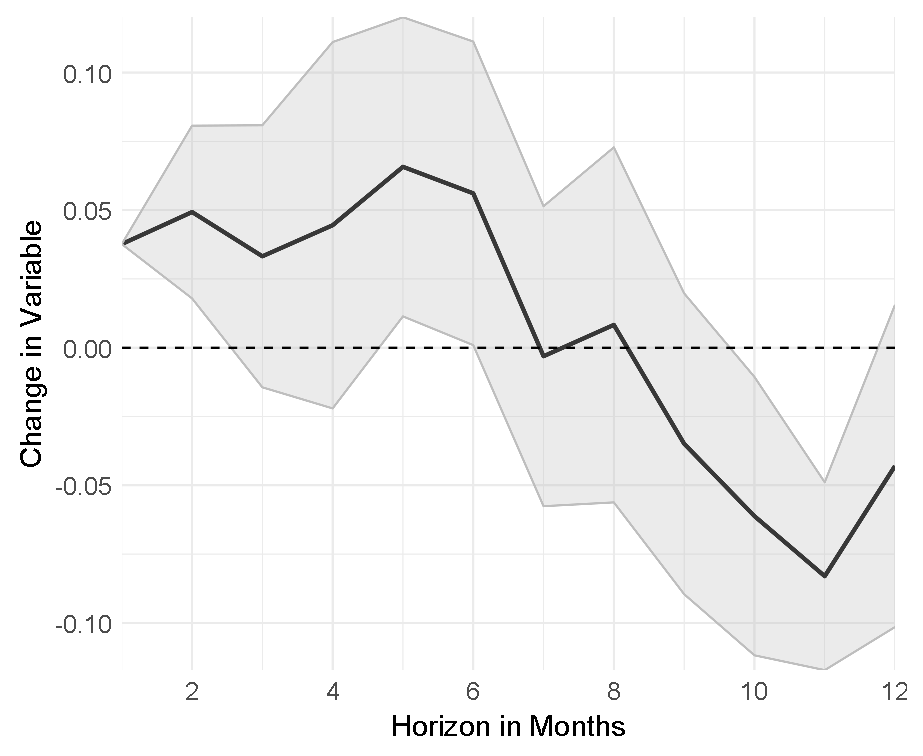
\includegraphics[width=1\textwidth]{output/lp/baseline/bHP/monetary_policy/monetary_policyonexpectations1y_djn.eps}
		\caption{Monetary policy on 1-year}
	\end{subfigure}
	\begin{subfigure}{00.32\textwidth}
		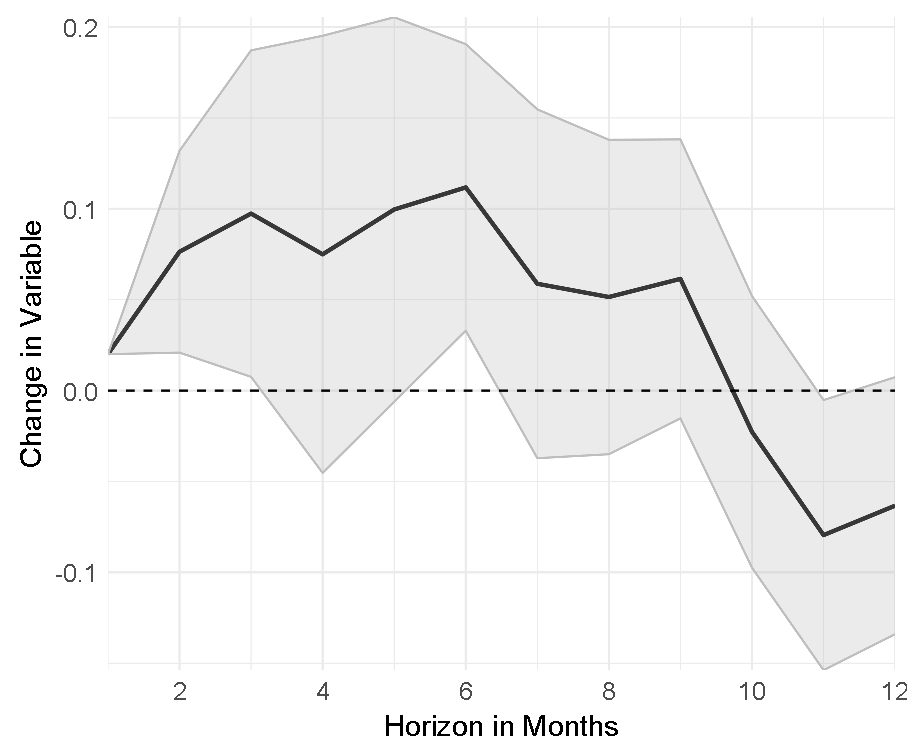
\includegraphics[width=1\textwidth]{output/lp/baseline/bHP/supply_chain/supply_chainonexpectations1y_djn.eps}
		\caption{Supply chain on 1-year}
	\end{subfigure}
	\begin{subfigure}{00.32\textwidth}
		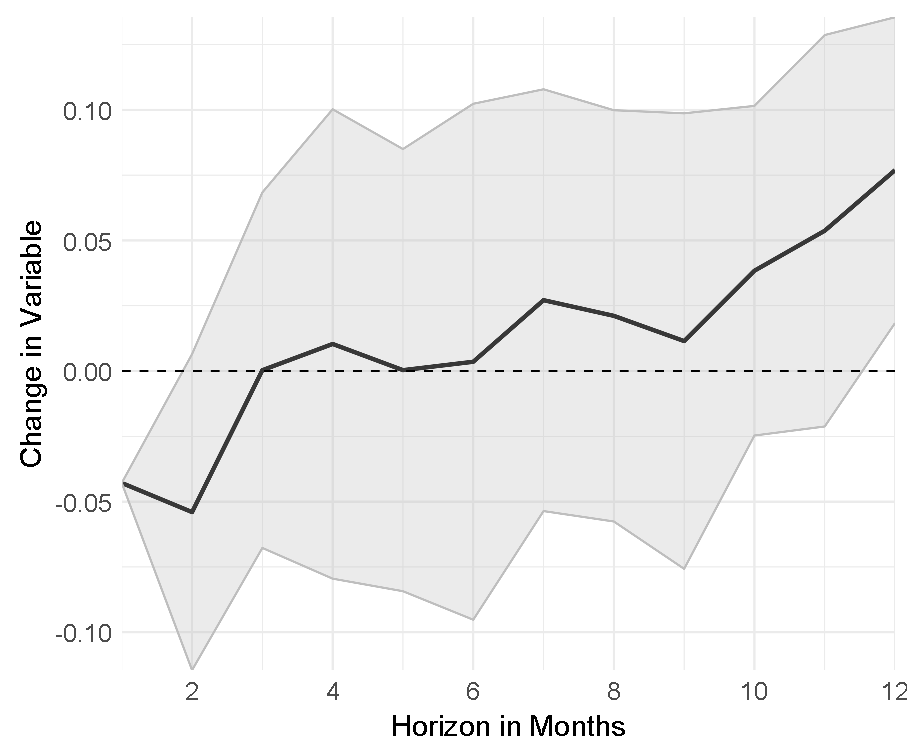
\includegraphics[width=1\textwidth]{output/lp/baseline/bHP/pandemic/pandemiconexpectations1y_djn.eps}
		\caption{Pandemic on 1-year}
	\end{subfigure}
	\begin{subfigure}{00.32\textwidth}
		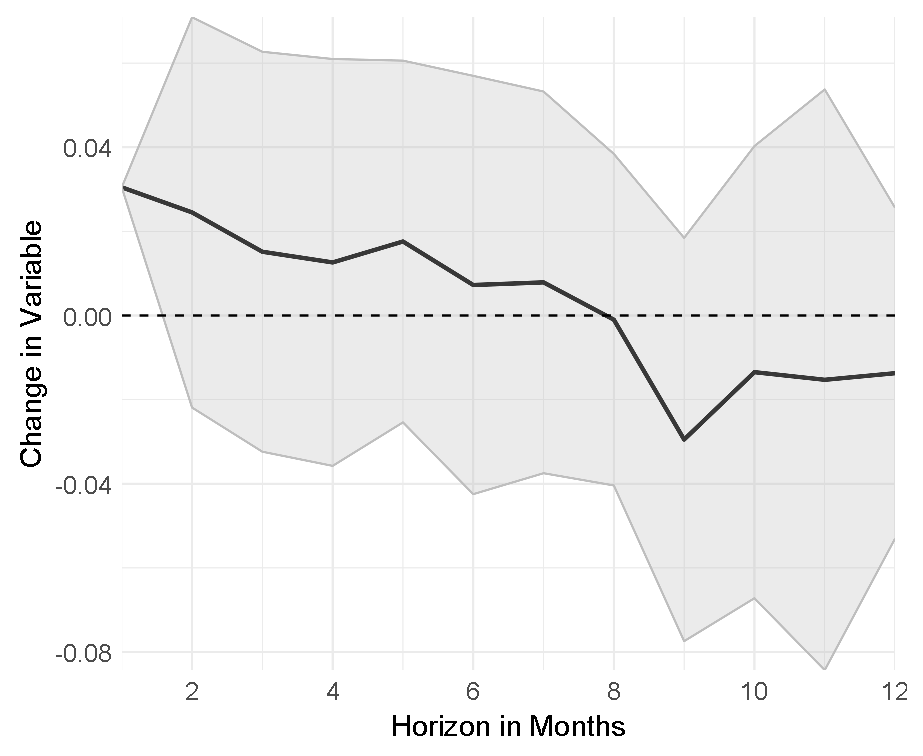
\includegraphics[width=1\textwidth]{output/lp/baseline/bHP/politics/politicsonexpectations3y_djn.eps}
		\caption{Politics on 3-year}
	\end{subfigure}
	\begin{subfigure}{00.32\textwidth}
		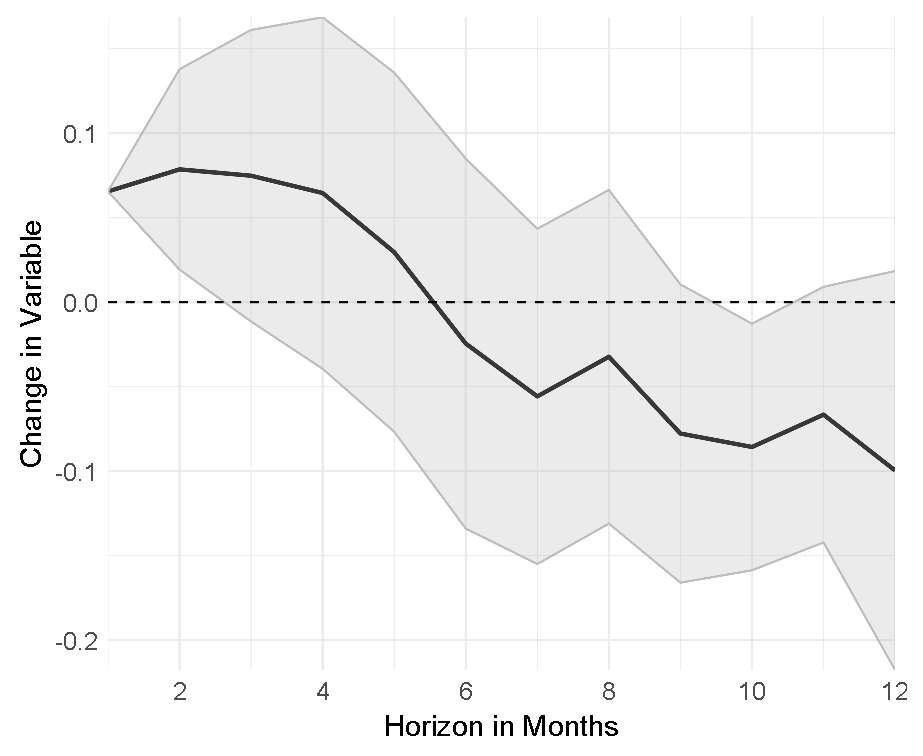
\includegraphics[width=1\textwidth]{output/lp/baseline/bHP/war/waronexpectations1y_djn.eps}
		\caption{War on 1-year}
	\end{subfigure}
	\begin{subfigure}{00.32\textwidth}
		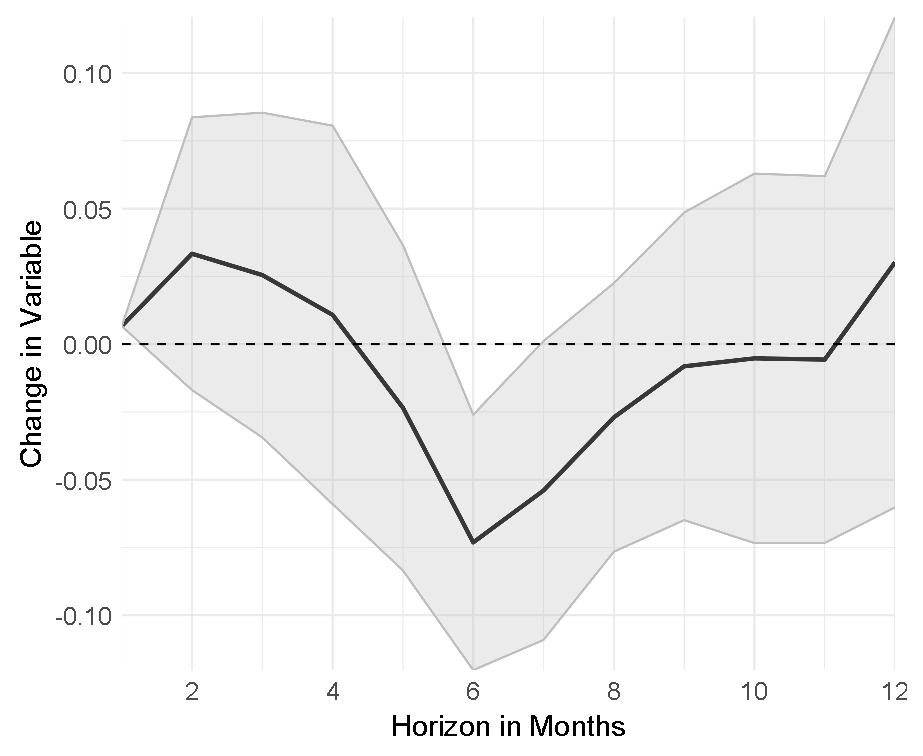
\includegraphics[width=1\textwidth]{output/lp/baseline/bHP/war/waronexpectations3y_djn.eps}
		\caption{War on 3-year}
	\end{subfigure}
	\begin{subfigure}{00.32\textwidth}
		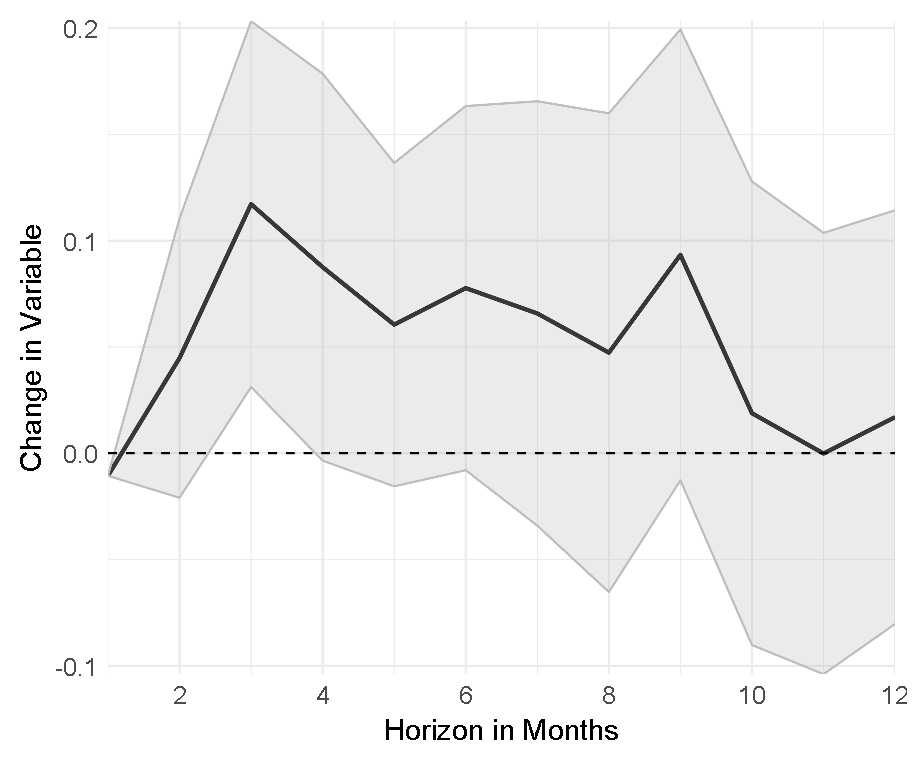
\includegraphics[width=1\textwidth]{output/lp/baseline/bHP/profits/profitsonexpectations1y_djn.eps}
		\caption{Profits on 1-year}
	\end{subfigure}
	\begin{subfigure}{00.32\textwidth}
		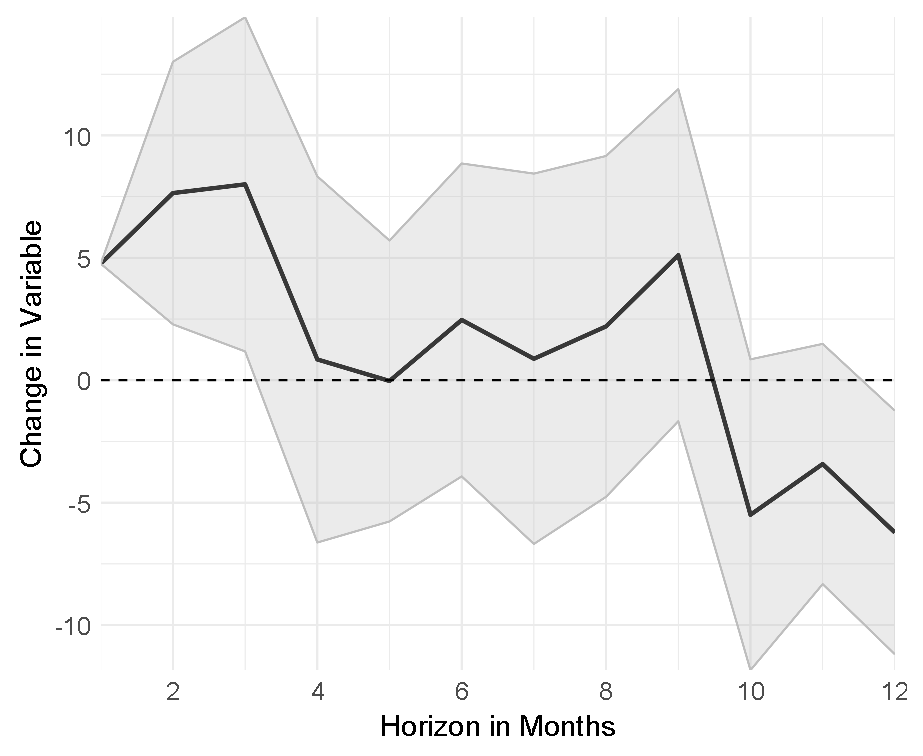
\includegraphics[width=1\textwidth]{output/lp/baseline/bHP/profits/profitsonexpectations3y_djn.eps}
		\caption{Profits on 3-year}
	\end{subfigure}
	\caption{Selection of narratives' impulse responses}
	\label{fig:irf_base}
	\floatfoot{Note: The graphs show the mean responses and 90\% confidence bands. The x-axis shows months (s) after narrative diffusion event; t = 0 is the month of the shock event. The y-axis shows the change in expectations as a response to the shock event. The shock considered is of the size of one standard deviation.}
\end{figure}
